Due to the presence of numerous physical, chemical, and physiological processes, vascular flow represents a highly complex process. In many cases, however, a simplified model that neglects some characteristics suffices for its description \cite{Saloner2019}. In this section, we briefly discuss key physiological considerations in blood flow modeling.

\section*{\fontsize{11}{15}\selectfont Vessel compliance}
The interaction between blood flow and elastic vessel walls can be modeled using methods such as the immersed boundary method \cite{Peskin}. In many cases wall elasticity can be neglected without significantly impacting results. Particularly in smaller vessels, neglecting the elasticity of the vascular walls has not shown a significant effect on the outcome. \cite{DempereMarco2006} However, this is not always the case, as significant non-negligible effects on the overall error of the results have been observed in the area of the aorta when considering rigid geometry \cite{LANTZ2011}. Generally, neglecting elasticity in larger vessels can introduce notable errors.

Note that including the elasticity of vascular walls in the considered model requires appropriately defining the  fluid-structure interaction, which is generally a difficult task in vascular flow, often depending heavily on accurate \textit{in vivo} measurements. Additionally, in diseases such as arteriosclerosis\footnote{Arteriosclerosis is a disease in which the arterial walls thicken and subsequently lose their elasticity \cite{Fishbein2015}.}, vessels lose their elasticity, thus including elasticity in the model may not necessarily reflect the physiological state of the vessels correctly \cite{Saloner2019}.

\section*{\fontsize{11}{15}\selectfont Blood viscosity}
Blood is often modeled as a Newtonian fluid. However, there are situations where the Newtonian behavior of blood is compromised. In cases where the flow velocity of blood is very low, red blood cells can aggregate, which leads to increased the viscosity of blood. Areas with such low flow velocities can be found, e.g., in regions of aneurysmal dilation\footnote{Aneurysmal dilation is a condition characterized by localized enlargement of a blood vessel \cite{Syed1997}.}. Conversely, the viscosity significantly decreases in areas where blood flows through very narrow vessels, particularly through vessels at the scale of arterioles or capillaries \cite{Saloner2019}.

Multiple viscosity models aim to capture the physiological behavior of blood viscosity more accurately~\cite{Saloner2019, Eichler2023, Boyd2007}. The simplest is the Power law model \cite{Sequeira} defining the viscosity as
\begin{equation}\label{eq:power-law}
	\mu _{\text{PL}} (\dot{\gamma}) = C_p  \dot{\gamma} ^{n_1-1} \ ,
\end{equation}
where $ C_p$ \si{[kg.m^{-1}]} and $ n_1 $ \si{[-]} are empirical parameters. Another model is the Casson model \cite{Boyd2007} which satisfies
\begin{equation}\label{eq:Casson}
	\mu _{\text{CA}} (\dot{\gamma}) = \frac{1}{\dot{\gamma}} \left[ k_{0} + k_{1} \sqrt{\dot{\gamma}} \right]^2 \ ,
\end{equation}
where $ k_1$ \si{[kg^{2}.m^{-2}]} and $ k_2 $ \si{[kg^{2}.m^{-2}]} are empirically determined constants. A disadvantage of these two simple models is their limited applicability, as they fail for shear rates approaching zero \cite{Boyd2007}.

Among the more complex models, the Cross model \cite{Sequeira} is defined by the relation
\begin{equation}\label{eq:cross}
	\mu _{\text{CR}} (\dot{\gamma}) = \frac{\mu_{0} - \mu_{\infty}}{1 + (k\dot{\gamma})^{n_2}} + \mu_{\infty}  \ ,
\end{equation}
where $ k $ \si{[s]} and $ n_2 $ \si{[-]} are constants, and
\begin{equation}\label{eq:m0 a minf}
	\mu _{0}  = \lim_{\dot{\gamma} \rightarrow 0+}\mu (\dot{\gamma})\, , \ \mu_{\infty} = \lim_{\dot{\gamma} \rightarrow \infty}\mu (\dot{\gamma}).
\end{equation}
The last model we mention is the Carreau-Yasuda model \cite{Boyd2007} satisfying
\begin{equation}\label{eq:C-Y}
	\mu _{\text{CY}} (\dot{\gamma}) = \mu_{\infty} + (\mu_{0} - \mu_{\infty}) \left[ 1 + (\varepsilon \dot{\gamma}) ^{a} \right]^{\frac{n_3-1}{a}} \ ,
\end{equation}
where $ \varepsilon$ \si{[s]} , $a$ \si{[-]}, and $ n_3 $ \si{[-]} are empirically determined constant parameters that influence the model behavior between boundary viscosity values. For $ \mu_{0}$ and $ \mu_{\infty} $ \eqref{eq:m0 a minf} applies.

All listed models are compared in Figure~\ref{fig:vs}, with the parameter values taken from \cite{Eichler2023}.
\begin{figure}[h]
	\centering
	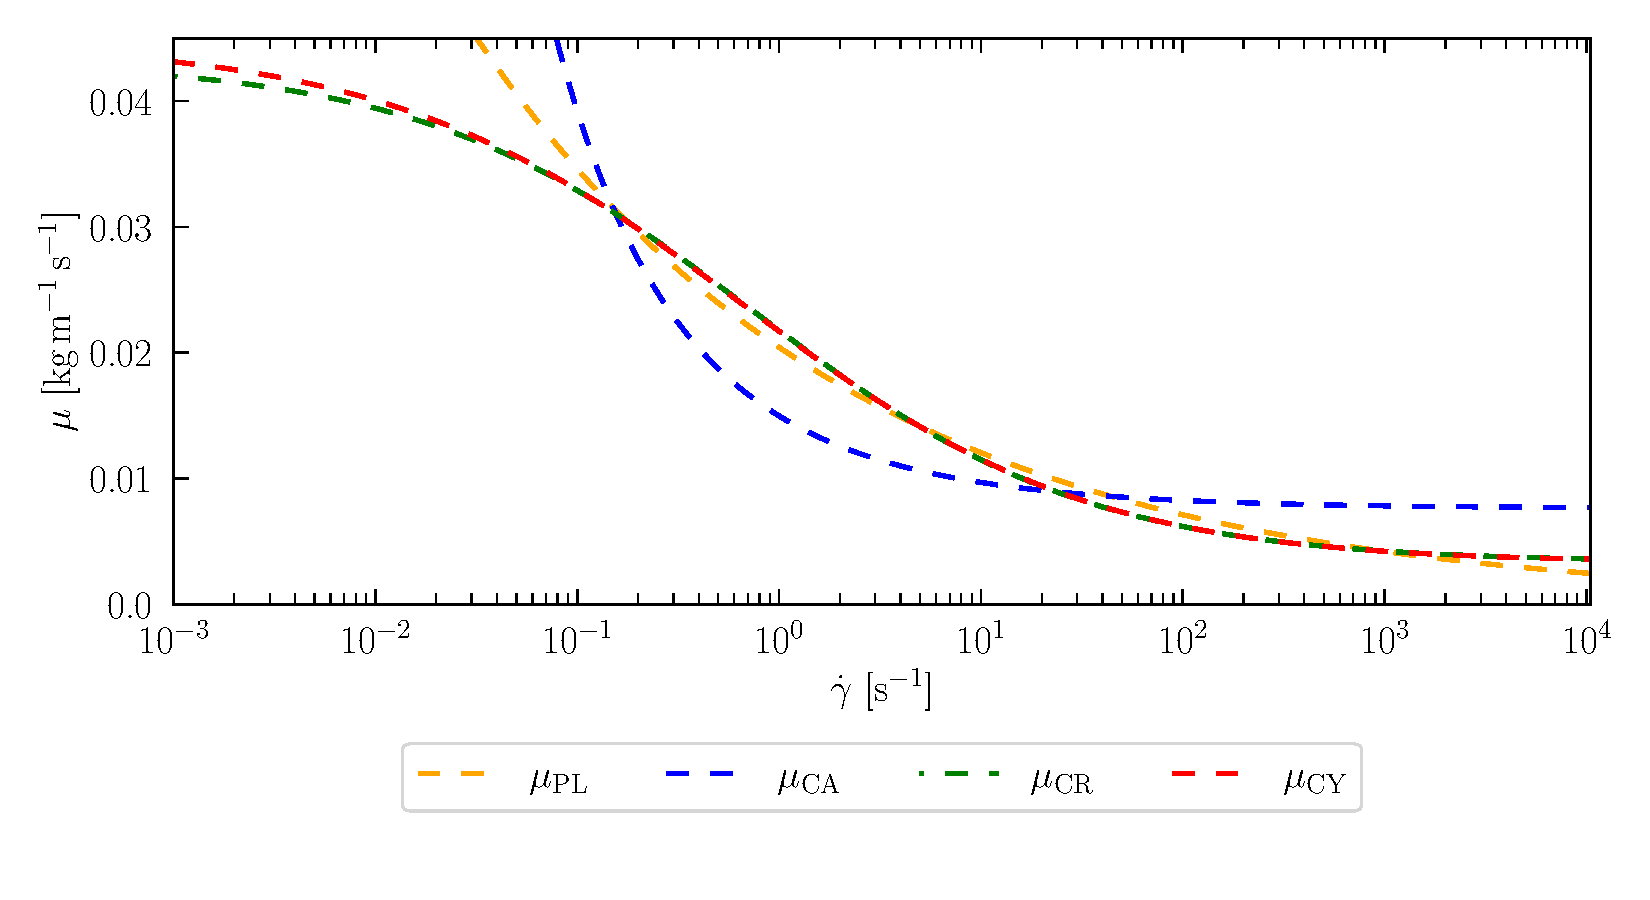
\includegraphics[width=1.0\textwidth]{figures/modely.pdf}
	\caption{Comparison of non-Newtonian viscosity models, specific parameter values were taken from~\cite{Eichler2023}. Each model is denoted in correspondence with the defining equations
		\eqref{eq:power-law}, \eqref{eq:Casson}, \eqref{eq:cross}, and \eqref{eq:C-Y}.}
	\label{fig:vs}
\end{figure}

\section*{\fontsize{11}{15}\selectfont Turbulent flow}
Blood flow is mostly laminar under normal physiological conditions \cite{Sequeira}. However, turbulent flow can occur in specific situations \cite{Saqr2020}. One notable region where turbulence is frequently observed is behind a vascular stenosis\footnote{Vascular stenosis is a condition characterized by localized narrowing of a blood vessel \cite{Carabello2009}.} \cite{Jain2022}. The flow velocity of blood in the narrowed region can significantly increase. Although the flow typically remains laminar within the narrowed part of the vessel, the increased velocity downstream can lead to the formation of vortices and changes in the flow regime \cite{Sequeira, Saloner2019, Varghese2003}.

The occurrence of turbulent flow is physiologically undesirable, as it is often results in significant dissipation of kinetic energy, increasing the strain on the circulatory system. Furthermore, regions with turbulent flow show increased stress on the vessel walls, which can contribute to tissue damage and increased risk of developing conditions such as arteriosclerosis \cite{Saloner2019, Kameneva2004}.